% NOTE - this is only a template without real arguments
\begin{entry}{Log API test: tightening up}{April 9, 2021}
    \objective 
    
    Further updates on the log test, including the lookup table for headers, adding timecodes, and fixing some stuff.
    I forgot to update this for a couple weeks so this will contain quite a few different small updates.
    \outline
    
    \begin{enumerate}
        \item Find a way to update the .csv header with  real names rather than MRIDs
        \item Find a way to add the simulation timecode as a column
        \item Convert the simulation timecode to an actual datetime
    \end{enumerate}
    
    \procedures
    
        \section{Header}
            The output stream provides a dictionary of dictionaries, each sub-dictionary containing values associated with
            a measurement id (MRID). These MRIDs are a CIM thing that are associated not just with measurements but with
            models, components, etc. I needed a way to take these MRIDs and turn them into names so the logs are reasonable.
            In order to do this, I needed to use one of the queries to get a list of MRIDs with names, and write a script
            in the callback function to automate converting MRIDs to names for the header (but, importantly, not the csvwriter
            object's header! Otherwise the writer stops working.) This is done.

        \section{Add timecodes}
            This is a little more dry. I am taking timecodes from the logging topic, putting them in an array each
            time the callback function is called, and adding that to the .csv output. I needed a snippet to get the
            column on the left. This works well enough, except at the end I realized this contains the CURRENT date
            and time, not the SIMULATION date and time. So I need to rewrite this to get the right thing.

        \section{Readable timecodes}
            This was a pain and took a long while until I realized pandas does it natively. I convert the GAD timecodes
            (which are in a unix-like format but with extra digits for ms) to dates and times using pandas. I should
            really just use pandas for everything on the rewrite.



    \results
    
    Mostly, except the timecodes are wrong. I just need to modify the script so that \verb"SIMULATION_TIME" reads from the
    output stream rather than the logging stream, I think.
    
\end{entry}


%\begin{entry}{CMake Error running EGOT-DCM Dockerfile}{Dec 02, 2020}
%    \objective
%
%    Determine the cause of the CMake error while running the dockerfile and modify file to get it to successfully build.
%
%    \outline
%
%    \begin{itemize}
%        \item Try running to see if it was just Lorry or a machine issue.
%        \item If it is a machine issue, modify configurations to ensure interoperability.
%        \item If I get the error track down its cause and modify dockerfile to fix.
%        \item Repeat until all builds are successful.
%    \end{itemize}
%
%    \procedures
%
%    \begin{itemize}
%        \item \mint{console}|git clone https://github.com/EGoT-DCS-SunSpec-Modbus|
%        \item \mint{console}|docker build -f Dockerfile.buster -t egot-dcs .|
%        \item \mint{console}|docker container run -i egot-dcs|
%    \end{itemize}
%
%    \observations
%
%    \begin{error}{Cmake Error: No CMAKE\_CXX\_COMPILER found}
%        \begin{figure}[H]
%            \centering
%            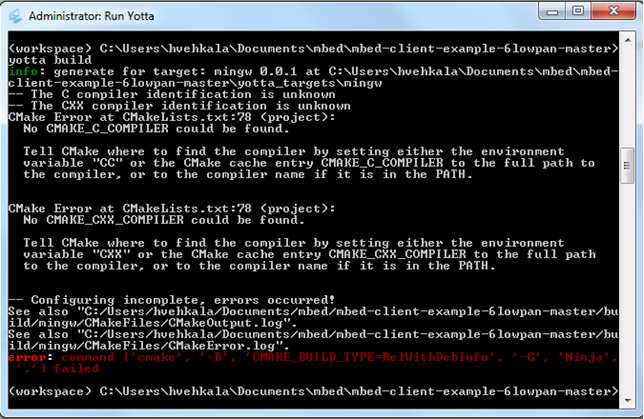
\includegraphics[height=4in]{Fall2020/Figures/cmake_error.png}
%        \end{figure}
%
%        Solution: what you need to do found at \cite{CMAKE-Forum}
%    \end{error}
%
%    \results
%
%    Short: No.
%
%    Long: Well...
%
%
%\end{entry}